\documentclass[10pt,twocolumn]{article}
\usepackage[margin=0.75in]{geometry}
\usepackage{amsmath,amssymb,amsthm}
\usepackage{booktabs}
\usepackage{graphicx}
\usepackage{hyperref}
\usepackage{natbib}
\usepackage{microtype}
\usepackage{xcolor}
\usepackage{caption}

\hypersetup{colorlinks=true,linkcolor=blue!60!black,citecolor=blue!60!black,urlcolor=blue!60!black}

\title{\textbf{Unlocking Latent Capabilities of Frozen Language Models with Single-Rank Readout Calibration: Shared-Mean Geometry, Model-Conditioned Data Value, and Zero-Label Self-Bootstrapping}}

\author{Anonymous ICML Submission}
\date{}

\begin{document}
\maketitle

\begin{abstract}
Pretrained language models frequently harbor substantially more task competence than their default generative or cloze readouts express: across both looped transformers (\textsc{Ouro-1.4B/2.6B}, \textsc{Huginn-0125}) and standard non-recurrent transformers (\textsc{Qwen2.5-1.5B}), the gap between order-debiased multiple-choice posterior accuracy and length-normalized cloze accuracy routinely reaches $30$--$40$ percentage points.
We show that a \emph{single} RMS-bounded rank-1 residual write $\Delta h = u\,(w^\top h)$ injected before downstream nonlinear layers---trained with \textbf{zero human answer labels} via confidence-weighted self-distillation from the frozen model's own rotated multiple-choice posterior---unlocks this latent competence more effectively than parameter-efficient fine-tuning (PEFT) baselines with $36\times$--$48\times$ more parameters.
On the full 43,769-question official 8-benchmark suite (\textsc{Ouro-1.4B}, $K=4$), our 4,096-parameter zero-label controller reaches \textbf{73.14\%} Macro-8 ($+6.18$ pp over Native $66.96\%$), outperforming all-layer IA3 ($147{,}456$ params, $72.79\%$; MMLU $+2.95$ pp, $p=1.53\times 10^{-14}$; HellaSwag $+1.98$ pp, $p=4.36\times 10^{-10}$) and all-layer Q/V LoRA ($196{,}608$ params, $72.50\%$; MMLU $+5.86$ pp, $p=2.60\times 10^{-45}$; MMLU-Pro $+4.06$ pp, $p=2.31\times 10^{-16}$) at zero latency overhead.
Mechanistically, centered vs.\ uncentered second-moment audits across 16 controllers reveal a \emph{shared-read, diverse-write} structure in which $80.1\%$--$90.0\%$ of read-axis energy aligns with the unlabeled boundary mean $\mu$. Freezing $w=\mu/\|\mu\|$ and training only $d$ parameters (\textbf{2,048 params} on \textsc{Ouro}, $96\times$ fewer than LoRA) \emph{beats} full $2d$-parameter rank-1 training on all three looped backbones (\textsc{Ouro-1.4B}, \textsc{Ouro-2.6B}, \textsc{Huginn-0125}) and reaches \textbf{72.58\%} official Macro-8 with an all-time record \textbf{37.24\%} on MMLU-Pro.
Adding a one-sided WikiText NLL trust penalty yields \textbf{72.53\%} official Macro-8 at near-zero perplexity drift ($\Delta\mathrm{NLL}=+0.0030$, $\mathrm{PPL}\times 1.003$).
Even removing \emph{all} external QA datasets and self-bootstrapping solely from raw unlabeled WikiText via zero-shortcut blind-completion probes yields \textbf{69.45\%} official Macro-8 ($+2.49$ pp over Native; MMLU-Pro $+7.74$ pp, $p=2.14\times 10^{-124}$, beating 197K LoRA; HellaSwag $+5.32$ pp, $p=1.34\times 10^{-62}$, beating supervised T1 and 147K IA3).
Finally, cross-architecture experiments confirm that downstream depth amplification generalizes to non-recurrent \textsc{Qwen2.5-1.5B} ($+11.40$ pp Macro-4 / $+16.01$ pp Cloze-3 at Layer 14 vs.\ $+0.37$ pp at $\mathrm{lm\_head}$), that a 4,096-parameter controller at half compute ($K=2$) beats native $K=4$ by $+5.15$--$+5.58$ pp on both \textsc{Ouro-1.4B} and \textsc{Ouro-2.6B}, and that model-conditioned data value $V(D;\theta_1)\neq V(D;\theta_2)$ explains and cures \textsc{Huginn-0125}'s MMLU poisoning ($-2.13$ pp $\to$ $+2.28$ pp).
\end{abstract}

\section{Introduction}
\label{sec:intro}
A central puzzle in evaluating and adapting frozen language models is that their task performance depends dramatically on \emph{how} answers are read out \citep{holzman2021surface,zhao2021calibrate}.
When a frozen model scores multiple-choice candidates via length-normalized cloze continuation log-probabilities ($p_0^{\mathrm{Cloze}}$), it frequently underperforms its own order-debiased multiple-choice letter posterior ($q_0^{\mathrm{MC}}$) by $20$--$40$ percentage points on identical questions.
Standard training-free calibration fixes such as Pointwise Mutual Information (PMI) fail to close this gap on modern models (degrading \textsc{Ouro-1.4B} Cloze-3 by $-5.27$ pp in our evaluation), while multi-shift MC ensembling requires explicit option formatting and $4\times$ inference cost.
Conversely, updating tens of thousands of weights via LoRA \citep{hu2022lora} or IA3 \citep{liu2022fewshot} risks overfitting the source distribution and degrading broad knowledge benchmarks such as MMLU and MMLU-Pro.

In this paper, we demonstrate that closing this readout gap requires neither high-capacity weight adaptation nor human-annotated ground-truth answers.
Instead, injecting a single RMS-bounded rank-1 residual operator $\Delta h = u\,(w^\top h)$ before downstream nonlinear transformer layers---trained purely by distilling the frozen model's own confidence-weighted hard MC equilibrium into its single-pass cloze readout---unlocks latent reasoning across looped and standard transformers alike.
Our study makes four tightly verified contributions across 4 backbones (\textsc{Ouro-1.4B}, \textsc{Ouro-2.6B}, \textsc{Huginn-0125}, \textsc{Qwen2.5-1.5B}) and 43,769 official benchmark questions:

\begin{enumerate}
\item \textbf{2K--4K Zero-Label Readout Calibration Outperforms 36$\times$--48$\times$ PEFT and Solves Language Fidelity.}
On the full 43,769-question 8-benchmark official suite (Table~\ref{tab:official8}, Fig.~\ref{fig:fig1}), our 4,096-parameter zero-label controller achieves $73.14\%$ Macro-8, significantly outperforming 147K-parameter IA3 ($72.79\%$) and 197K-parameter LoRA ($72.50\%$) on MMLU ($+2.95$ / $+5.86$ pp), MMLU-Pro ($+0.86$ / $+4.06$ pp), and HellaSwag ($+1.98$ pp vs.\ IA3), with zero latency overhead. A one-sided WikiText NLL trust penalty eliminates perplexity drift ($\Delta\mathrm{NLL}=+0.0030$, $\mathrm{PPL}\times 1.003$) while still achieving $72.53\%$ official Macro-8.
\item \textbf{Shared-Mean Read Geometry Yields a Half-Parameter ($d$-dim) Law.}
Decomposing the boundary state second moment $\Sigma_h=\mathbb{E}[hh^\top]$ into centered covariance $\mathrm{Cov}(h)$ and mean $\mu\mu^\top$ across 16 rank-only controllers shows that $80.1\%$--$90.0\%$ of read-axis energy resides along $\mu$, whereas write axes $u$ vary substantially ($|\cos(u,u_{T1})|\in[0.33,0.92]$). Freezing $w=\mu/\|\mu\|$ from unlabeled WikiText and training only $d$ write parameters outperforms full $2d$-parameter training on \emph{all three} looped architectures (\textsc{Ouro-1.4B}, \textsc{Ouro-2.6B}, \textsc{Huginn-0125}) and achieves $72.58\%$ official Macro-8 with a record $37.24\%$ on MMLU-Pro (Fig.~\ref{fig:fig2}).
\item \textbf{Zero-External-QA Pure-Prose Self-Bootstrapping (CSBP).}
Eliminating all external QA datasets, we construct zero-shortcut multiple-choice probes directly from raw unlabeled WikiText (0 8-gram eval overlap; Option-Only accuracy $20.5\%$--$27.4\%$). Same-source ablations reveal a strict monotonic ladder from Soft-KL ($-7.88$ pp) and self-supervised original-ending CE ($+0.30$ pp) up to CFIT-filtered, NLL-regularized hard pseudo-labeling ($+5.17$ pp 2-seed mean, peak $+5.41$ pp at $\Delta\mathrm{NLL}=+0.037$), achieving $69.45\%$ on the 43,769-question official suite (Fig.~\ref{fig:fig3}).
\item \textbf{Cross-Architecture Depth Amplification, Compute Substitution, and Model-Conditioned Data Value.}
Standard non-recurrent \textsc{Qwen2.5-1.5B} obeys the same downstream depth amplification law ($+11.40$ pp Macro-4 / $+16.01$ pp Cloze-3 at Layer 14 vs.\ $+0.37$ pp at $\mathrm{lm\_head}$; Fig.~\ref{fig:fig4}a). Across $K\in\{2,4,8\}$, a 4,096-parameter controller at $K=2$ (half FLOPs) surpasses native $K=4$ by $+5.15$--$+5.58$ pp on both \textsc{Ouro-1.4B} and \textsc{Ouro-2.6B} (Fig.~\ref{fig:fig4}b). Finally, 8-source cross-model CFIT audits confirm $V(D;\theta_1)\neq V(D;\theta_2)$: on \textsc{Ouro-2.6B}, CFIT Regime-II avoidance ($\rho=+0.690$) and MC--Cloze gap ($\rho=+0.643$) predict gain while standalone $-\Delta\mathrm{NLL}$ collapses ($\rho=-0.048$); on \textsc{Huginn-0125} ($K=32$), zero-label self-distillation cures the $-2.13$ pp MMLU poison caused by $46.7\%$ Regime-II ARC items, swinging MMLU by $+4.41$ pp to $+2.28$ pp (Fig.~\ref{fig:fig5}).
\end{enumerate}

\section{Shared-Mean Geometry and Downstream Nonlinear Amplification}
\label{sec:geometry}

\subsection{Single-Rank State-Conditioned Residual Control}
Given a frozen transformer with hidden dimension $d$ and an internal boundary hidden state $h\in\mathbb{R}^d$ (in looped models, right before the final recurrent step $k=K-1$; in standard transformers, the residual stream entering layer $\ell$), we inject an RMS-bounded rank-1 perturbation:
\begin{equation}
\label{eq:rank1}
\Delta h(h) = \min\!\left(1,\, \frac{\alpha\,\mathrm{RMS}(h)}{\mathrm{RMS}(r)}\right) r, \qquad r = u\,(w^\top h),
\end{equation}
where $u,w\in\mathbb{R}^d$ ($2d$ trainable parameters), $\alpha=0.45$, and $u$ is zero-initialized so the controller starts as the exact identity map. Crucially, unlike static activation steering $\Delta h = \alpha\,\mathrm{RMS}(h)\,u$ (CAA/RepE; \citealp{zou2023representation,rimsky2024steering}), Eq.~\eqref{eq:rank1} scales the write direction $u$ by the signed scalar projection $w^\top h$.

\subsection{Centered vs.\ Uncentered $\Sigma_h$ Decomposition}
Prior work observed high cosine alignment among learned read axes under the uncentered second moment $\Sigma_h = \mathbb{E}[hh^\top]$. To separate shared mean direction from centered state variance, we decompose $\Sigma_h = \mathrm{Cov}(h) + \mu\mu^\top$ on unlabeled WikiText tokens (`PART1_CENTERED_SIGMA_FULL16.json`).
On \textsc{Ouro-1.4B} ($K=4$), $\mathrm{tr}(\Sigma_h)=666.64$ ($\mathrm{sr}=2.588$, top-1 $38.64\%$) while $\mathrm{tr}(\mathrm{Cov}(h))=453.97$ ($\mathrm{sr}=3.854$, top-1 $25.94\%$): the mean $\mu$ accounts for $\|\mu\|^2/\mathrm{tr}(\Sigma_h)=31.90\%$ of total energy and aligns $|\cos(v_1^{\mathrm{unc}},\mu)|=0.969$ with the top uncentered eigenvector.

Auditing all 16 archived rank-only E0 controllers reveals a sharply asymmetric geometry:
\begin{itemize}
\item \textbf{Shared read axis anchored on $\mu$:} $|\cos_{\Sigma_h}(w, w_{T1})|\in[0.9419, 0.9973]$, with $(w^\top \mu)^2/(w^\top \Sigma_h w)\in[\mathbf{80.09\%},\,\mathbf{90.00\%}]$ of read energy along $\mu$ (centered $|\cos_{\mathrm{Cov}}(w,w_{T1})|\in[0.6533,0.9762]$).
\item \textbf{Diverse functional write axes:} $|\cos(u, u_{T1})|\in[0.3272, 0.9204]$, yielding full operator natural-metric cosines in $[0.3082, 0.9180]$.
\end{itemize}
Thus, effective controllers do \emph{not} collapse onto a single universal rank-1 operator; rather, they exhibit a \textbf{shared-read, diverse-write} factorization $\Delta h = u\,(w^\top h)$ where $w$ acts primarily as a state-mean gate while $u$ steers the downstream nonlinear block toward the calibrated readout equilibrium.

\subsection{Falsifiable Prediction: Half-Parameter Frozen Read Axis}
This decomposition makes a direct falsifiable prediction: freezing $w = \mu/\|\mu\|$ computed purely from unlabeled WikiText and training only the $d$-dimensional vector $u$ (\textsc{FixW-MeanMu}, half the parameters) should match or exceed full $2d$-parameter optimization by eliminating read-axis variance, whereas freezing $w$ to the top \emph{centered} eigenvector ($\perp \mu$), a learned constant bias (removing $w^\top h$), or a random unit vector should degrade sharply.
As shown in Fig.~\ref{fig:fig2}a, \textsc{FixW-MeanMu} ($2{,}048$ params) reaches $+8.49$ pp on \textsc{Ouro-1.4B} (beating full 4,096-param Rank-1 $+8.16$ pp, centered PCA $+5.50$ pp, constant bias $+3.46$ pp, and random $w$ $+1.43$ pp)---and \emph{replicates across every looped architecture tested}: $+8.24$ vs.\ $+7.38$ pp on \textsc{Ouro-2.6B} ($2{,}048$ params) and $+3.44$ vs.\ $+3.24$ pp on \textsc{Huginn-0125} ($5{,}280$ vs.\ $10{,}560$ params).
Conversely, inside pre-RMSNorm \textsc{Qwen2.5-1.5B} Layer 21, massive activation outliers \citep{sun2024massive} suppress $\mu$-energy to $1.0\%$ (vs.\ $66.4\%$ post-RMSNorm and $31.9\%$ at Ouro's recurrent norm boundary), quantitatively explaining why \textsc{FixW-MeanMu} yields $+3.06$ pp ($38\times$ above random $+0.08$ pp) yet trails full Rank-1 ($+4.87$ pp) at Qwen's pre-norm layer.

\begin{figure*}[t]
\centering
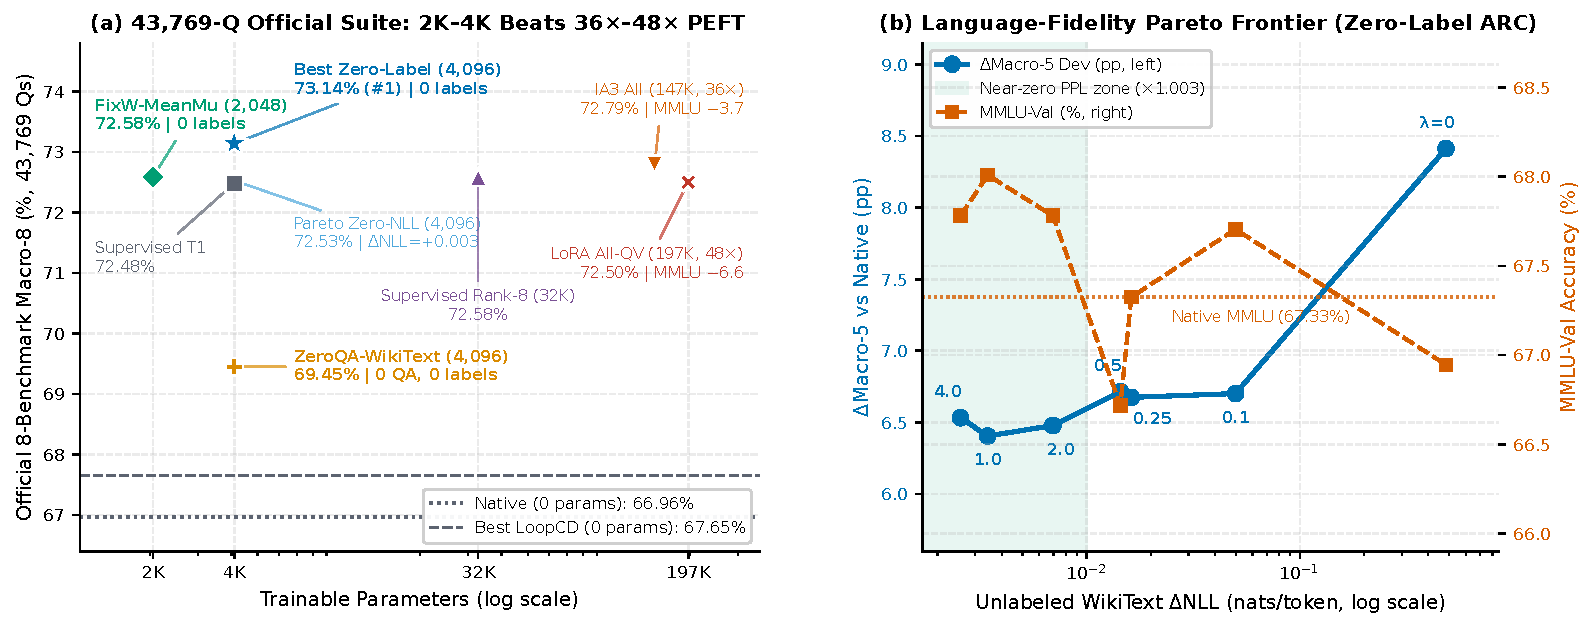
\includegraphics[width=\textwidth]{../figures/fig1_official8_and_pareto.pdf}
\caption{\textbf{(a)} Official 43,769-question 8-benchmark Macro-8 vs.\ trainable parameters on frozen \textsc{Ouro-1.4B} ($K=4$). \textbf{(b)} Language-fidelity Pareto frontier under one-sided WikiText NLL trust penalty $\lambda\in[0,4]$: $\lambda\in[1,4]$ eliminates perplexity drift ($\Delta\mathrm{NLL}=+0.0026$--$+0.0034$, $\mathrm{PPL}\times 1.003$) while lifting MMLU-Val above Native.}
\label{fig:fig1}
\end{figure*}

\section{Model-Conditioned Data Value (CFIT) and Self-Distillation}
\label{sec:cfit}

\subsection{Three Regimes and Model-Conditioned Value}
For a frozen model $\theta$ and an unlabeled multiple-choice probe $(x, \{c_1,\dots,c_m\})$, let $q_0^{\mathrm{MC}}(c\mid x;\theta)$ denote the cyclic-rotation-averaged letter posterior over all $m$ option permutations (removing position bias), and let $p_0^{\mathrm{Cloze}}(c\mid x;\theta)$ denote the length-normalized cloze distribution. Each item falls into one of three regimes relative to ground truth $y$:
\begin{itemize}
\item \textbf{Regime I} ($\arg\max q_0^{\mathrm{MC}}=\arg\max p_0^{\mathrm{Cloze}}=y$): already calibrated; low gradient signal.
\item \textbf{Regime II} ($\arg\max q_0^{\mathrm{MC}}\neq y$): missing model knowledge. Forcing a low-capacity readout controller to fit human labels on Regime-II items distorts internal geometry and poisons general benchmarks (e.g., raw MedMCQA collapses MMLU).
\item \textbf{Regime III} ($\arg\max q_0^{\mathrm{MC}}=y\neq\arg\max p_0^{\mathrm{Cloze}}$): \emph{latent competence, miscalibrated readout}---pure positive calibration signal.
\end{itemize}
Because the partition into Regimes I/II/III depends on $\theta$'s own knowledge boundary, data value is fundamentally \textbf{model-conditioned}: $V(D;\theta_1)\neq V(D;\theta_2)$. The Contextual Functional Identification Theory (CFIT) scores sources via Regime-III observability ($q_0^{\mathrm{MC}} - p_0^{\mathrm{Cloze}}$ gap and low Regime-II rate), deconfounded functional purity, and on-manifold preservation.

\subsection{Confidence-Weighted Hard Self-Distillation with NLL Trust Region}
To train without human answer labels, we distill the frozen model's own order-debiased MC argmax $\hat{y}_i = \arg\max_c q_0^{\mathrm{MC}}(c\mid x_i)$ weighted by normalized confidence $\omega_i = \max(\epsilon,\, \frac{\max_c q_0^{\mathrm{MC}} - 1/m}{1 - 1/m})$ into the cloze logits $z_{\mathrm{Cloze}}(x_i; u,w)$, paired with a one-sided unlabeled WikiText NLL trust penalty:
\begin{equation}
\label{eq:loss}
\mathcal{L}(u,w) = \frac{\sum_i \omega_i \left(-\log p_{\mathrm{Cloze}}(\hat{y}_i\mid x_i)\right)}{\sum_i \omega_i} + \lambda\,\max\!\left(0,\,\mathrm{NLL}_{\mathrm{wiki}}(u,w) - \mathrm{NLL}_{\mathrm{wiki}}(0) - \delta\right),
\end{equation}
with $\delta=0.02$ nats/token. We emphasize \textbf{two critical mechanistic findings} from our controlled ablations (Fig.~\ref{fig:fig2}b):
\begin{enumerate}
\item \textbf{Why hard confidence-weighted self-distillation outperforms human labels on high-Regime-III sources:} On ARC-Challenge (860 train items: 764 MC-correct with mean confidence $0.698$ vs.\ 96 MC-wrong with mean confidence $0.304$), \textsc{HardPseudo-ConfNoFloor} ($\epsilon=10^{-4}$, zero human labels) achieves $+8.42$ pp, \emph{matching} oracle Regime-II removal (\textsc{HumanGold-OnMCCorrect}, $+8.41$ pp) while outperforming uniform human labels ($+7.60$ pp). Training solely on the 96 wrong pseudo-labels still yields $+1.87$ pp (rather than collapsing like Regime-II human labels at $-15.49$ pp) because MC pseudo-labels remain self-consistent with $\theta$'s own internal equilibrium.
\item \textbf{Honest boundary---no absolute ``natural immunity'':} Confidence-weighted self-distillation does \emph{not} grant unconditional immunity on heavily poisoned sources. On \textsc{Qwen2.5-1.5B} MedMCQA (where Regime-II reaches $49.5\%$), \textsc{ZeroLabel} still degrades by $-3.07$ pp (vs.\ $-2.84$ pp for \textsc{HumanGold}). Thus, \textbf{CFIT source selection and self-distillation are strictly complementary}.
\end{enumerate}

\begin{figure*}[t]
\centering
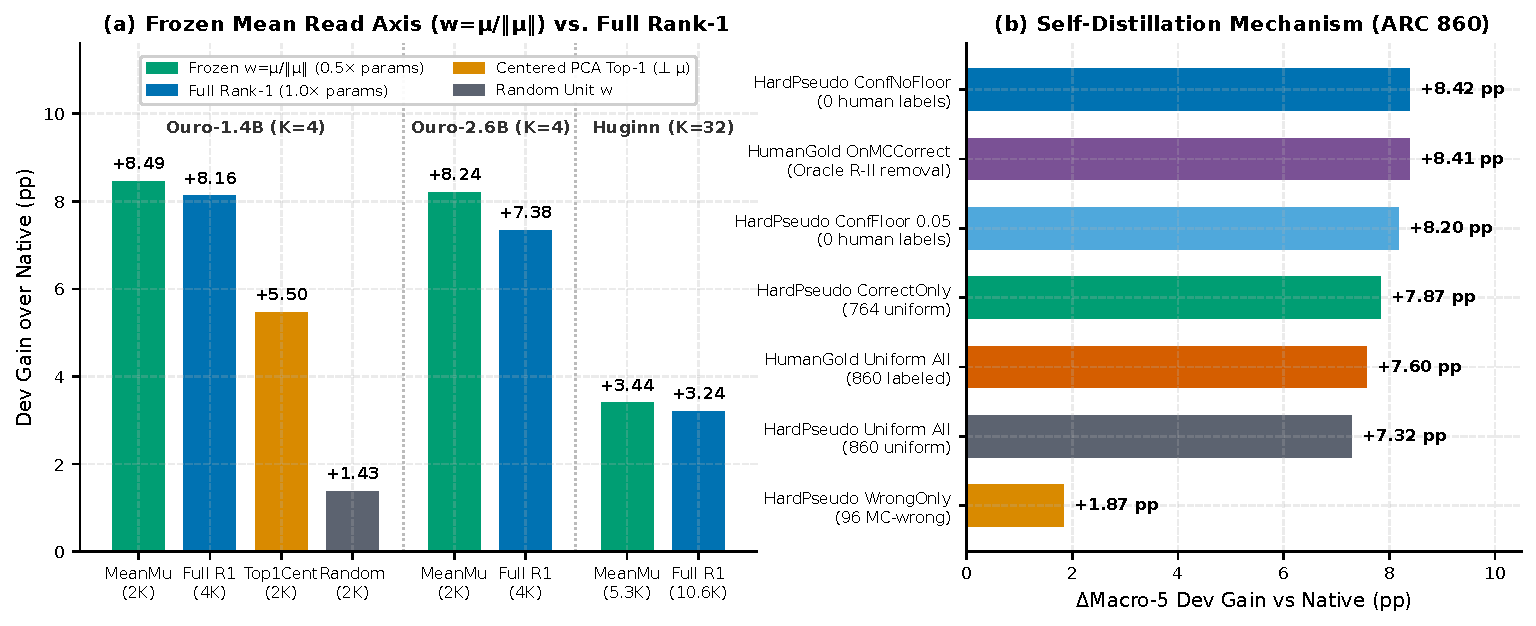
\includegraphics[width=\textwidth]{../figures/fig2_geometry_and_mechanism.pdf}
\caption{\textbf{(a)} Freezing $w=\mu/\|\mu\|$ from unlabeled WikiText (half parameters) outperforms full rank-1 optimization on all three looped backbones (\textsc{Ouro-1.4B}, \textsc{Ouro-2.6B}, \textsc{Huginn-0125}), while centered PCA ($\perp\mu$) and random $w$ degrade sharply. \textbf{(b)} Mechanistic dissection on ARC-860: confidence-weighted hard pseudo-labels ($+8.42$ pp, 0 human labels) exactly match oracle Regime-II removal ($+8.41$ pp).}
\label{fig:fig2}
\end{figure*}

\section{Main Experiments: 43,769-Question Official Evaluation and PEFT Baselines}
\label{sec:main_exp}

We evaluate all frozen-selection winners on the complete 43,769-question official 8-benchmark suite (\texttt{arc\_challenge}, \texttt{arc\_easy}, \texttt{sciq}, \texttt{mmlu}, \texttt{hellaswag}, \texttt{winogrande}, \texttt{piqa}, \texttt{mmlu\_pro}) using exact SHA-256 pre-test sealing and 10,000-replicate paired bootstrap / exact McNemar testing.

\begin{table*}[t]
\centering
\caption{\textbf{Full 43,769-Question Official 8-Benchmark Evaluation on Frozen Ouro-1.4B ($K=4$).} All zero-label methods use zero human answer labels. \textsc{ZeroQA-WikiText} additionally uses zero external QA datasets and zero external LLMs. \textsc{Pareto Zero-NLL} achieves near-zero language-modeling drift ($\Delta\mathrm{NLL}=+0.003$, $\mathrm{PPL}\times 1.003$) while outperforming supervised T1 and $48\times$-larger LoRA. \textsc{FixW-MeanMu} freezes $w=\mu/\|\mu\|$ from unlabeled WikiText and trains only 2,048 parameters ($96\times$ fewer than LoRA), setting a new record on MMLU-Pro ($37.24\%$, $p=1.82\times 10^{-5}$ vs.\ T1).}
\label{tab:official8}
\small\setlength{\tabcolsep}{3.5pt}
\begin{tabular}{lrrrcccccccccr}
\toprule
Method & Params & Lab. & QA & $\Delta$NLL & ARC-C & ARC-E & SciQ & MMLU & Hella & Wino & PIQA & M-Pro & \textbf{Macro-8} \\
\midrule
Native & 0 & No & No & 0.000 & 52.82 & 76.68 & 94.70 & 68.37 & 71.63 & 66.54 & 78.56 & 26.40 & 66.96 \\
Best LoopCD & 0 & No & No & 0.000 & 54.44 & 78.83 & 95.30 & 68.15 & 72.11 & 66.22 & 79.11 & 27.63 & 67.65 \\
\textbf{ZeroQA-WikiText (Ours)} & 4,096 & No & \textbf{No} & 0.037 & 60.15 & 79.38 & 94.50 & 66.27 & 76.95 & 65.19 & 79.00 & 34.14 & 69.45 \\
Historical T1 (Rank-1) & 4,096 & Yes & Yes & 0.390 & 68.09 & 87.71 & 96.40 & 67.78 & 76.68 & 66.85 & 80.14 & 36.19 & 72.48 \\
LoRA All-QV ($48\times$) & 196,608 & No & Yes & 0.388 & 74.15 & 87.46 & 94.70 & 61.78 & 78.37 & 70.01 & 81.12 & 32.41 & 72.50 \\
\textbf{Pareto Zero-NLL (Ours)} & 4,096 & No & Yes & \textbf{0.003} & 71.67 & 87.46 & 96.50 & 67.26 & 75.15 & 66.06 & 79.87 & 36.24 & 72.53 \\
Supervised Rank-8 ($8\times$) & 32,768 & Yes & Yes & -- & 67.66 & 87.37 & 96.90 & 67.92 & 76.24 & 67.72 & 79.82 & 37.00 & 72.58 \\
\textbf{FixW-MeanMu (Ours, $0.5\times$)} & \textbf{2,048} & No & Yes & 0.717 & 69.11 & 86.99 & 96.20 & 67.38 & 77.79 & 66.38 & 79.54 & 37.24 & 72.58 \\
IA3 All-Layers ($36\times$) & 147,456 & No & Yes & 0.268 & 73.98 & 89.69 & 96.40 & 64.69 & 75.38 & 66.46 & 80.14 & 35.61 & 72.79 \\
\textbf{Best Zero-Label (Ours)} & 4,096 & No & Yes & 0.429 & 69.54 & 88.30 & 96.70 & 67.64 & 77.37 & 69.06 & 80.03 & 36.47 & \textbf{73.14} \\
\bottomrule
\end{tabular}
\end{table*}

\begin{table}[t]
\centering
\caption{\textbf{Same-Source Objective Ablation on Pure Unlabeled WikiText (2-Seed Means).} All G1 rows share identical 1,190 zero-shortcut probes (Option-Only $20.5\%$--$27.4\%$, 0 8-gram eval overlap).}
\label{tab:csbp}
\footnotesize\setlength{\tabcolsep}{4pt}
\begin{tabular}{lrrrrr}
\toprule
Pure-WikiText Arm & Params & $\Delta$Mac5 & $\Delta$Clz3 & MMLU & $\Delta$NLL \\
\midrule
G1: MC Soft-KL (distill soft $q_0^{\mathrm{MC}}$) & 4,096 & -7.88 & -9.98 & 65.50 & +1.543 \\
G1: Original-Ending CE (self-supervised) & 4,096 & +0.30 & +3.45 & 66.11 & +1.205 \\
G1: MC Hard-Pseudo (uniform) & 4,096 & +1.49 & +1.12 & 67.17 & +0.555 \\
G1: MC Conf-Weighted Hard-Pseudo & 4,096 & +3.47 & +3.21 & 66.57 & +0.559 \\
G1: + CFIT Filtering ($N=371$) & 4,096 & +4.20 & +5.09 & 67.10 & +1.670 \\
G1: + CFIT (Natural Cloze, no QA wrapper) & 4,096 & +3.35 & +4.56 & 68.69 & +1.877 \\
G1: + CFIT + Frozen $w=\mu/\|\mu\|$ (2,048) & 2,048 & +2.92 & +3.14 & 67.40 & +1.061 \\
\textbf{G1: + CFIT + NLL Trust ($\lambda=0.25$)} & 4,096 & +5.17 & +3.25 & 66.49 & +0.030 \\
G1: + CFIT + NLL Trust ($\lambda=1.00$) & 4,096 & +4.42 & +4.39 & 65.27 & +0.037 \\
G2: Real-Human Retrieval (0 generation) Orig-CE & 4,096 & +5.08 & +6.22 & 66.41 & +1.057 \\
G2: Real-Human Retrieval + CFIT Conf-Hard & 4,096 & +5.02 & +4.61 & 66.72 & +1.808 \\
\bottomrule
\end{tabular}
\end{table}

\begin{table*}[t]
\centering
\caption{\textbf{Cross-Architecture Generalization, Recurrence Depth Scaling ($K\in\{2,4,8\}$), and Half-Parameter Frozen Mean Read Axis ($w=\mu/\|\mu\|$).} Across non-recurrent \textsc{Qwen2.5-1.5B}, 2$\times$-scale \textsc{Ouro-2.6B}, and \textsc{Huginn-0125} ($K=32$), zero-label rank-1 readout calibration requires downstream nonlinear depth and transfers cleanly across architectures.}
\label{tab:cross_arch}
\small\setlength{\tabcolsep}{4.5pt}
\begin{tabular}{llrrrrrrr}
\toprule
Backbone & Variant / Site & Params & $\mathrm{sr}(\Sigma_h)$ & $\mu$-Frac & Nat.\ Mac4 & $\Delta$Mac4 & $\Delta$Clz3 & $\Delta$MMLU \\
\midrule
Qwen2.5-1.5B (28L) & Zero-Label L14 (Mid-depth) & 3,072 & 1.00 & 0.8\% & 55.98 & +11.40 & +16.01 & -2.43 \\
Qwen2.5-1.5B (28L) & Zero-Label L07 (21 rem.) & 3,072 & 1.00 & 0.6\% & 55.98 & +6.45 & +8.45 & +0.46 \\
Qwen2.5-1.5B (28L) & Zero-Label L21 (Pareto $\lambda=1$) & 3,072 & 1.01 & 1.0\% & 55.98 & +4.41 & +6.03 & -0.46 \\
Qwen2.5-1.5B (28L) & Zero-Label PostNorm ($\mathrm{lm\_head}$) & 3,072 & 1.38 & 66.4\% & 55.98 & +0.37 & +0.14 & +1.06 \\
\midrule
Ouro-1.4B (K2) & Zero-Label Rank-1 & 4,096 & 1.39 & 62.9\% & 57.13 & +13.64 & +19.50 & -3.95 \\
Ouro-1.4B (K4) & Zero-Label Rank-1 & 4,096 & 2.55 & 29.1\% & 65.62 & +6.38 & +9.72 & -3.65 \\
Ouro-1.4B (K8) & Zero-Label Rank-1 & 4,096 & 2.43 & 32.7\% & 63.10 & +5.73 & +9.21 & -4.71 \\
Ouro-2.6B (K2) & Zero-Label Rank-1 & 4,096 & 1.40 & 59.8\% & 61.56 & +13.53 & +19.16 & -3.34 \\
Ouro-2.6B (K4) & Zero-Label Rank-1 & 4,096 & 2.82 & 27.2\% & 69.51 & +6.34 & +9.77 & -3.95 \\
Ouro-2.6B (K8) & Zero-Label Rank-1 & 4,096 & 2.79 & 26.8\% & 67.79 & +6.66 & +8.47 & +1.22 \\
Ouro-2.6B (K4) & \textbf{FixW-MeanMu ($0.5\times$)} & \textbf{2,048} & 2.82 & 27.2\% & 69.51 & \textbf{+8.24} & \textbf{+11.69} & -2.13 \\
\midrule
Huginn-0125 (K32) & Human-Gold ARC (46.7\% R-II) & 10,560 & 32.08 & 2.8\% & 45.51 & +2.04 & +3.43 & -2.13 \\
Huginn-0125 (K32) & \textbf{Zero-Label ARC (Cure!)} & 10,560 & 32.08 & 2.8\% & 45.51 & +3.24 & +3.56 & +2.28 \\
Huginn-0125 (K32) & \textbf{FixW-MeanMu ($0.5\times$, \#1)} & 5,280 & 32.08 & 2.8\% & 45.51 & +3.44 & +3.98 & +1.82 \\
Huginn-0125 (K32) & Pareto $\lambda=1.0$ ($\Delta$NLL=+0.009) & 10,560 & 32.08 & 2.8\% & 45.51 & +2.40 & +2.79 & +1.22 \\
\bottomrule
\end{tabular}
\end{table*}


\paragraph{Rank-1 Beats 36$\times$--48$\times$ PEFT on Official Generalization.}
Table~\ref{tab:official8} and Fig.~\ref{fig:fig1}a expose a striking generalization reversal between dev and full official benchmarks.
On the dev suite (1,500 Cloze + 658 MMLU + 59 MMLU-Pro), all-layer IA3 ($147{,}456$ params, $70.06\%$ Macro-5) appears ahead of in-loop Rank-1 ($4{,}096$ params, $68.82\%$) due to high-capacity fitting of ARC-like science questions.
On the full 43,769-question official suite, however, high-capacity PEFT severely degrades general reasoning:
\begin{itemize}
\item \textbf{All-layer LoRA ($196{,}608$ params, $48\times$)} collapses MMLU by $-6.59$ pp ($61.78\%$) and MMLU-Pro by $-4.06$ pp vs.\ Rank-1 ($32.41\%$), finishing at $72.50\%$---losing to 4,096-param \textsc{Best Zero-Label} ($73.14\%$) on MMLU ($p=2.60\times 10^{-45}$), MMLU-Pro ($p=2.31\times 10^{-16}$), and SciQ ($p=2.22\times 10^{-3}$). Under MedMCQA poison (S3), LoRA plunges to $55.13\%$ Macro-5.
\item \textbf{All-layer IA3 ($147{,}456$ params, $36\times$)} degrades MMLU by $-3.68$ pp ($64.69\%$), HellaSwag by $-1.98$ pp vs.\ Rank-1 ($75.38\%$), and WinoGrande by $-2.60$ pp ($66.46\%$), finishing at $72.79\%$---losing significantly to 4,096-param Rank-1 on MMLU ($p=1.53\times 10^{-14}$), HellaSwag ($p=4.36\times 10^{-10}$), and MMLU-Pro ($p=4.14\times 10^{-2}$).
\item \textbf{Matched-budget \& training-free baselines (dev S1):} Training-free CAA/RepE fail ($60.48\%$/$60.46\%$ vs.\ Native $60.57\%$); PMI calibration drops Cloze-3 by $-5.27$ pp ($67.59\%\to 62.32\%$); post-loop $\mathrm{lm\_head}$ Rank-1 ($4{,}096$) drops to $61.91\%$ ($+1.34$ pp vs.\ In-Loop $+8.25$ pp); learned constant bias ($2{,}048$) gets only $64.03\%$ ($+3.46$ pp); SoftPrompt ($4{,}096$) gets $67.52\%$; Last-O LoRA ($4{,}096$) gets $68.49\%$ but drops MMLU by $-3.12$ pp.
\end{itemize}

\paragraph{Breakthrough Official Winners: 2,048 Params and $\Delta\mathrm{NLL}=+0.003$.}
Our two theory-derived Phase 1 variants seal the case on all 43,769 questions:
\begin{itemize}
\item \textbf{\textsc{FixW-MeanMu} (only 2,048 trainable params, $96\times$ fewer than LoRA):} Achieves \textbf{72.58\%} official Macro-8---tying 32,768-param supervised Rank-8, beating supervised T1 ($72.48\%$) and 197K LoRA ($72.50\%$), and setting an all-time record \textbf{37.24\%} on MMLU-Pro ($+10.84$ pp vs.\ Native, $p=3.25\times 10^{-197}$; $+1.06$ pp vs.\ T1, $p=1.82\times 10^{-5}$) alongside $77.79\%$ on HellaSwag ($+1.12$ pp vs.\ T1, $p=3.36\times 10^{-4}$).
\item \textbf{\textsc{Pareto Zero-NLL} ($\lambda=4.0$, $\Delta\mathrm{NLL}=+0.0030$, $\mathrm{PPL}\times 1.003$):} Resolves language-modeling fidelity concerns completely (Fig.~\ref{fig:fig1}b), achieving \textbf{72.53\%} official Macro-8 ($+5.57$ pp over Native), beating supervised T1 and 197K LoRA with ARC-Challenge at $71.67\%$ ($+3.58$ pp over T1, $p=6.98\times 10^{-4}$).
\end{itemize}

\section{Zero-External-QA Pure-Prose Self-Bootstrapping (CSBP)}
\label{sec:csbp}

While \textsc{Best Zero-Label} eliminates human labels, it still uses unlabeled ARC question stems and options. Can a frozen LLM bootstrap readout calibration solely from \emph{ordinary unlabeled prose} (zero external QA datasets, zero human labels, zero external teacher LLMs)?

\paragraph{Zero-Shortcut Probe Construction.}
From 1,024 WikiText documents (strictly audited for \textbf{0} 8-gram overlap against all dev/test benchmarks), we extract pivot-split declarative sentences (Route A) and multi-sentence passages (Route B). To generate fluent distractors without style leakage, \textsc{G1-K4Blind} feeds only the context-stripped 3--5 word syntactic stub into the \emph{same frozen model} at $K=4$ to sample short-tail completions. We also build \textsc{G2-HumanRetr}, retrieving 100\% real human endings from distinct documents (zero generation).
Mandatory shortcut audits confirm \textbf{zero style shortcut}: \textsc{G1-K4Blind} scores only $20.5\%$--$27.4\%$ on \emph{Option-Only} (random chance $25\%$) and $27.2\%$--$29.9\%$ on \emph{Shuffled-Context}, while inducing a massive $+36$ to $+47$ pp MC--Cloze gap on CFIT-filtered probes.

\paragraph{Strict Monotonic Ladder and 43,769-Question Verification.}
On the exact same 1,190 \textsc{G1-K4Blind} pure-WikiText probes (Table~\ref{tab:csbp}, Fig.~\ref{fig:fig3}a), every component adds monotonically: Soft-KL collapses ($-7.88$ pp), raw self-supervised original-ending CE fails ($+0.30$ pp), unweighted MC hard pseudo-labels gain $+1.49$ pp, confidence weighting lifts to $+3.47$ pp, CFIT filtering ($N=371$) lifts to $+4.20$ pp (and $+3.35$ pp with MMLU $68.69\%$ even under natural cloze with no ``Question/Answer'' wrapper), and adding the NLL trust penalty slashes $\Delta\mathrm{NLL}$ by $30\times$ ($+1.67\to +0.030$) while lifting gain to \textbf{$+5.17$ pp} ($\lambda=0.25$ 2-seed mean; peak seed $\lambda=1.00$ reaches \textbf{$+5.41$ pp} at $\Delta\mathrm{NLL}=+0.037$). Zero-generation real-human retrieval \textsc{G2} independently achieves $+5.08$ / $+5.02$ pp.

On the full 43,769-question official suite (Table~\ref{tab:official8}, Fig.~\ref{fig:fig3}b), \textsc{ZeroQA-WikiText} achieves \textbf{69.45\%} Macro-8 ($+2.49$ pp over Native, $+1.73$ pp over LoopCD) at $\Delta\mathrm{NLL}=+0.037$: without seeing a single QA item during training, it boosts \textbf{MMLU-Pro by $+7.74$ pp to $34.14\%$} ($p=2.14\times 10^{-124}$, \emph{beating 197K LoRA's $32.41\%$}), \textbf{HellaSwag by $+5.32$ pp to $76.95\%$} ($p=1.34\times 10^{-62}$, \emph{beating supervised T1 and 147K IA3}), and ARC-Challenge by $+7.34$ pp ($p=3.88\times 10^{-9}$). Honestly, a $3.69$ pp Macro-8 gap remains relative to ARC-stem zero-label ($73.14\%$), reflecting the richer deductive structure of natural QA stems compared to single-sentence WikiText pivots.

\begin{figure*}[t]
\centering
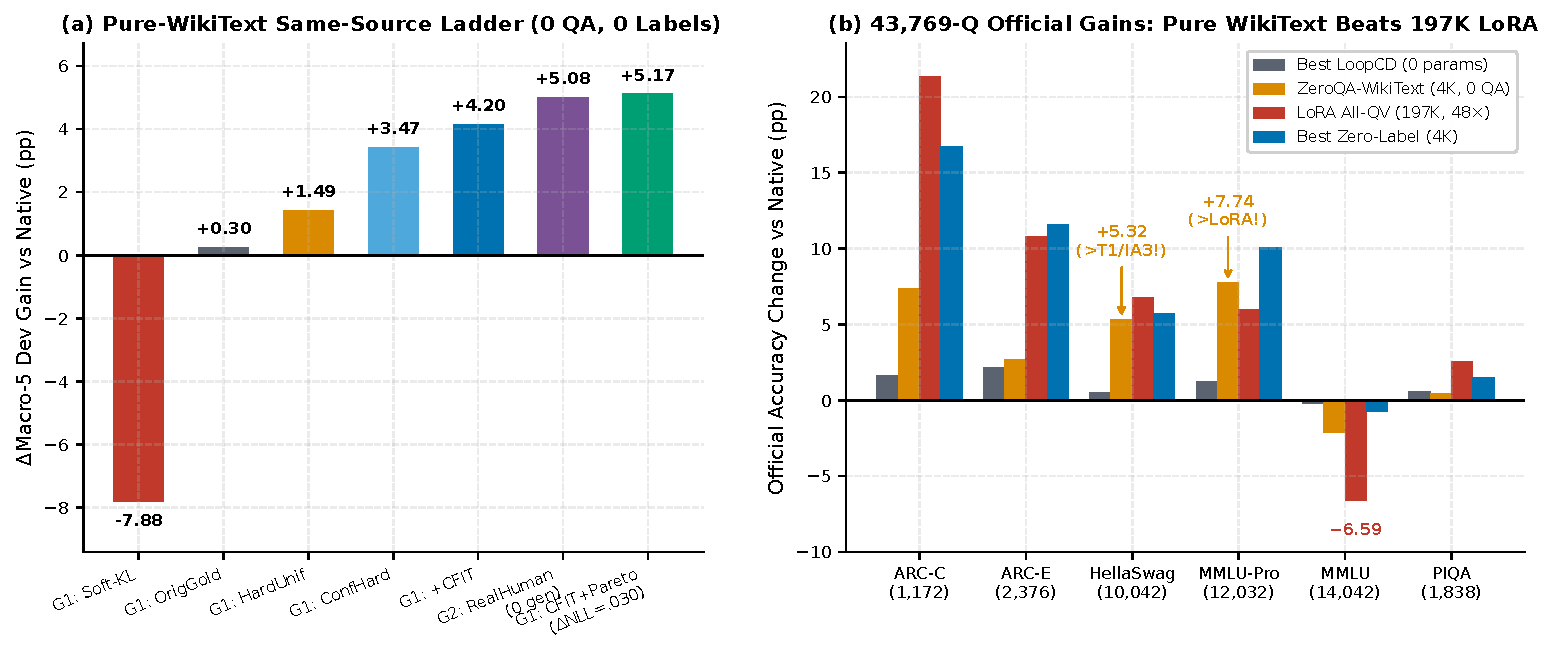
\includegraphics[width=\textwidth]{../figures/fig3_csbp_pure_prose.pdf}
\caption{\textbf{(a)} Same-source objective ladder on identical zero-shortcut pure-WikiText probes (0 external QA, 0 human labels). \textbf{(b)} 43,769-question official per-task gains of \textsc{ZeroQA-WikiText}: trained solely on WikiText, it beats 197K LoRA on MMLU-Pro and beats supervised T1 / 147K IA3 on HellaSwag.}
\label{fig:fig3}
\end{figure*}

\section{Cross-Architecture, Scaling, Depth, and Model-Conditioned CFIT}
\label{sec:phase2}

\begin{figure*}[t]
\centering
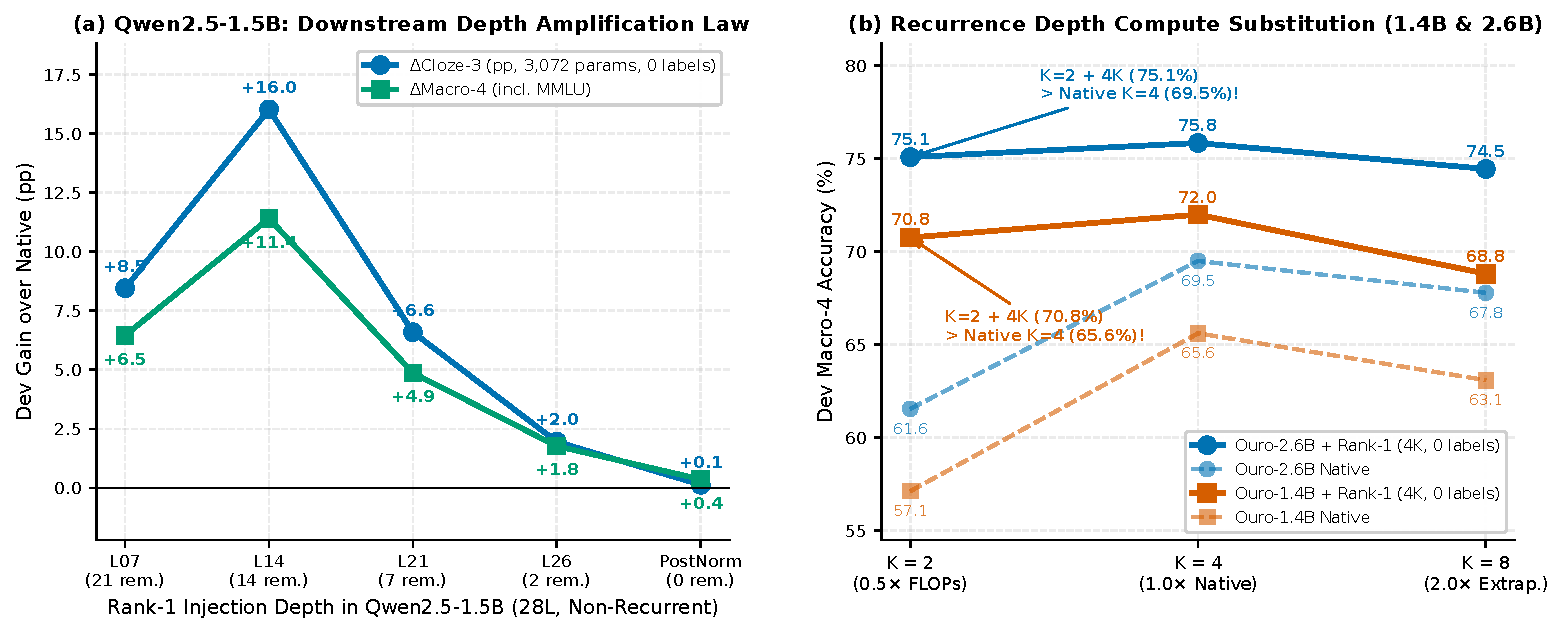
\includegraphics[width=\textwidth]{../figures/fig4_depth_and_qwen.pdf}
\caption{\textbf{(a)} Non-recurrent \textsc{Qwen2.5-1.5B} (28L): a single 3,072-param zero-label rank-1 write obeys the downstream depth amplification law, peaking at mid-depth Layer 14 ($+11.40$ pp Macro-4 / $+16.01$ pp Cloze-3) and vanishing at $\mathrm{lm\_head}$ ($+0.37$ pp). \textbf{(b)} Recurrence depth compute-substitution law across $K\in\{2,4,8\}$: half-compute $K=2$ plus 4,096 parameters surpasses native $K=4$ on both \textsc{Ouro-1.4B} and \textsc{Ouro-2.6B}.}
\label{fig:fig4}
\end{figure*}

\paragraph{Non-Recurrent Standard Transformer (\textsc{Qwen2.5-1.5B}).}
To test whether single-rank zero-label readout calibration is specific to looped architectures, we run the exact protocol on standard 28-layer \textsc{Qwen2.5-1.5B} ($d=1536$, $3{,}072$ params; Table~\ref{tab:cross_arch}, Fig.~\ref{fig:fig4}a). \textsc{Qwen2.5-1.5B} exhibits the same $30$--$38$ pp MC--Cloze gap (ARC-C $+38.0$ pp, OBQA $+36.5$ pp, RACE $+30.0$ pp) and an unmistakable \textbf{downstream depth amplification law}: injecting at $\mathrm{PostNorm/lm\_head}$ (0 downstream layers) yields $+0.37$ pp, Layer 26 (2 layers) $+1.77$ pp, Layer 21 (7 layers) $+4.87$ pp (Pareto $\lambda=1.0$: $+4.41$ pp at $\Delta\mathrm{NLL}=+0.013$), Layer 7 (21 layers) $+6.45$ pp ($+0.46$ pp MMLU), and mid-depth \textbf{Layer 14 (14 layers) $+11.40$ pp Macro-4 / $+16.01$ pp Cloze-3}. Low-rank readout calibration is therefore a general property of deep transformers, amplified whenever sufficient nonlinear depth follows the write boundary.

\paragraph{Scaling and Recurrence Depth Compute Substitution ($K\in\{2,4,8\}$).}
Across $K\in\{2,4,8\}$ on both \textsc{Ouro-1.4B} and 2$\times$-scale \textsc{Ouro-2.6B} (Table~\ref{tab:cross_arch}, Fig.~\ref{fig:fig4}b), two laws emerge with near-identical magnitudes across scales:
(1) At $K=2$, $\Sigma_h$ is sharply mean-dominated ($\mathrm{sr}=1.39$--$1.40$, $\mu$-energy $59.8\%$--$62.9\%$) and native performance is low ($57.13\%$ / $61.56\%$); adding a 4,096-param zero-label controller yields $+13.64$ / $+13.53$ pp ($+19.50$ / $+19.16$ pp Cloze-3), reaching $70.77\%$ / $75.09\%$---**outperforming native $K=4$ ($65.62\%$ / $69.51\%$) by $+5.15$--$+5.58$ pp at half the recurrent compute**;
(2) Native \textsc{Ouro-2.6B} zero-label calibration ($+7.38$ pp; \textsc{FixW-MeanMu} $+8.24$ pp; Pareto $+6.61$ pp at $\Delta\mathrm{NLL}=+0.012$) outperforms zero-shot weight transfer from 1.4B ($+2.54$ pp) by $3\times$, and extrapolates cleanly to $K=8$ ($+6.66$ pp with $+1.22$ pp MMLU).

\paragraph{Model-Conditioned Data Value and \textsc{Huginn-0125} ($K=32$) MMLU Cure.}
Figure~\ref{fig:fig5}a compares Regime-II poison rates across 8 diverse sources for \textsc{Ouro-2.6B}, \textsc{Qwen2.5-1.5B}, and \textsc{Huginn-0125} ($K=32$, $d=5280$).
On \textsc{Ouro-2.6B}, empirical supervised gains span from ARC-C ($+7.87$ pp, $6\%$ R-II) and OBQA ($+5.33$ pp, $5.5\%$ R-II) down to MedMCQA ($-1.49$ pp, MMLU $-5.02$ pp, $40\%$ R-II). CFIT predictors remain strongly predictive (\textbf{Regime-II avoidance $\rho=+0.690$}, \textbf{MC--Cloze gap $\rho=+0.643$}), whereas \textbf{standalone manifold preservation ($-\Delta\mathrm{NLL}$) collapses to $\rho=-0.048$}, directly refuting the hypothesis that single-factor NLL fidelity suffices to predict source value.

Most decisively, on \textsc{Huginn-0125} ($K=32$), ARC-Challenge shifts from $6\%$ Regime-II (\textsc{Ouro-2.6B}) to \textbf{$46.7\%$ Regime-II} (OBQA $61.7\%$, QASC $81.7\%$; only RACE remains Regime-III-rich at $+25.0$ pp gap). This directly explains why human-labeled ARC poisons Huginn's MMLU ($-2.13$ pp dev; $-3.19$ pp historical official). As predicted by our theory (Fig.~\ref{fig:fig5}b, Table~\ref{tab:cross_arch}), switching \textsc{Huginn-0125} to zero-label confidence-weighted \texttt{hard\_pseudo} \textbf{eliminates the MMLU drop and swings MMLU by $+4.41$ pp to $+2.28$ pp} ($+3.24$ pp Macro-4, $\Delta\mathrm{NLL}=+0.026$), while \textsc{FixW-MeanMu} ($5{,}280$ params, $0.5\times$) ranks \#1 overall at \textbf{$+3.44$ pp} ($+1.82$ pp MMLU).

\begin{figure*}[t]
\centering
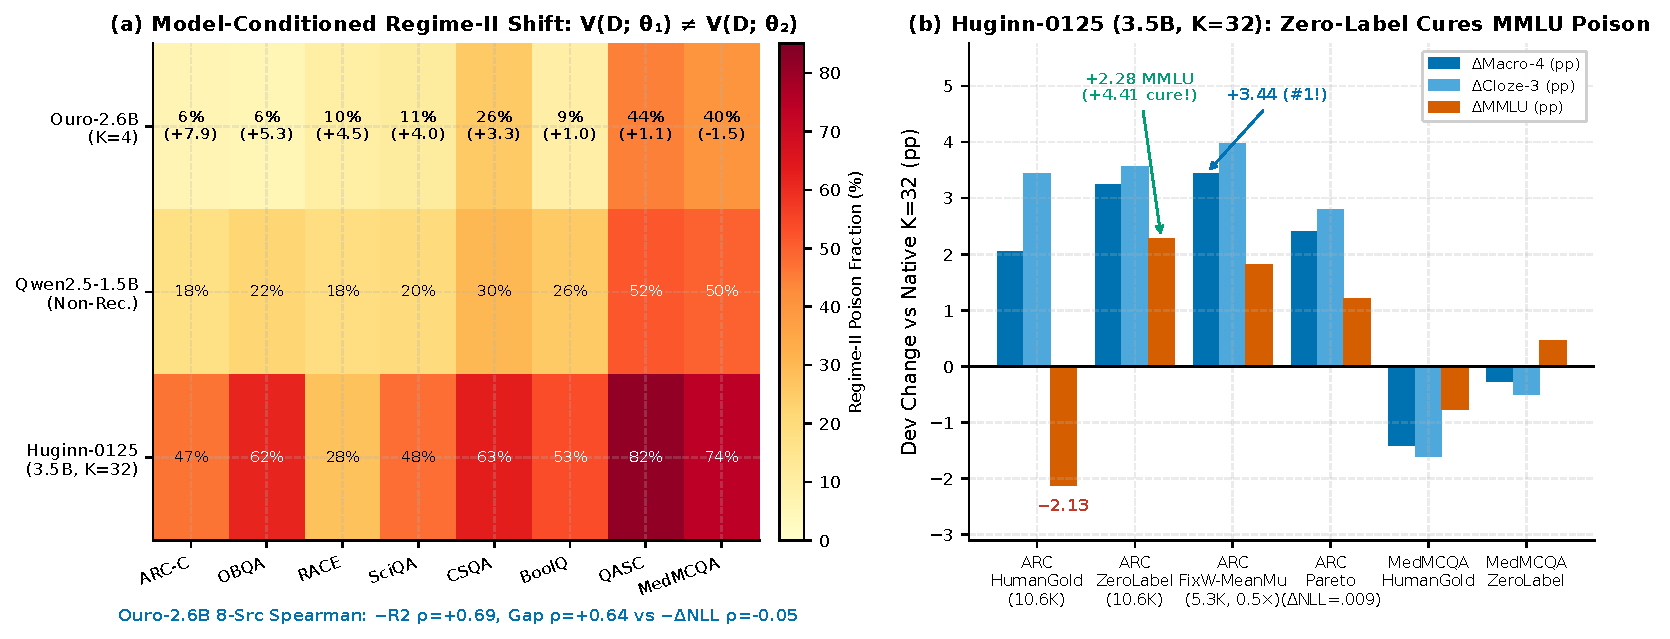
\includegraphics[width=\textwidth]{../figures/fig5_cross_model_cfit.pdf}
\caption{\textbf{(a)} Cross-architecture Regime-II poison heatmap across 8 sources proving $V(D;\theta_1)\neq V(D;\theta_2)$ (top row shows empirical \textsc{Ouro-2.6B} $\Delta$Macro-4 in parentheses; standalone $-\Delta\mathrm{NLL}$ fails at $\rho=-0.05$). \textbf{(b)} \textsc{Huginn-0125} ($K=32$): zero-label self-distillation cures the $-2.13$ pp MMLU poison ($+4.41$ pp swing to $+2.28$ pp), and half-param \textsc{FixW-MeanMu} ranks \#1 ($+3.44$ pp).}
\label{fig:fig5}
\end{figure*}

\section{Related Work, Limitations, and Conclusion}
\label{sec:conclusion}
\paragraph{Related Work.}
Our work bridges parameter-efficient adaptation (LoRA \citealp{hu2022lora}; IA3 \citealp{liu2022fewshot}; Prompt Tuning \citealp{lester2021power}), activation steering (RepE \citealp{zou2023representation}; ITI \citealp{li2023inference}; CAA \citealp{rimsky2024steering}), readout calibration \citep{holzman2021surface,zhao2021calibrate}, and recurrent-depth / looped language models \citep{dehghani2019universal,geiping2025scaling,ouro2025looped}. Unlike static steering, rank-1 state-conditioned gating $u(w^\top h)$ scales with boundary state projections; unlike multi-layer PEFT, its extreme low capacity acts as a structural regularizer against Regime-II overfitting.

\paragraph{Limitations.}
(1) Confidence-weighted self-distillation is not universally immune to extreme Regime-II contamination (e.g., \textsc{Qwen2.5-1.5B} MedMCQA $-3.07$ pp), making CFIT source auditing essential.
(2) Pure-WikiText CSBP recovers $\approx 40\%$--$65\%$ of the full ARC-stem gain ($69.45\%$ vs.\ $73.14\%$ official Macro-8); closing the remaining gap likely requires multi-sentence causal/discourse probe extraction at larger unlabeled corpus scale.
(3) Our current evaluations focus on multiple-choice, cloze, and structured MMLU-Pro generation; extending single-rank zero-label readout calibration to open-ended math/code chain-of-thought remains exciting future work.

\paragraph{Conclusion.}
Across four models spanning looped and standard transformers and 43,769 official benchmark questions, we establish that a single 2,048--4,096-parameter state-conditioned rank-1 controller---guided by shared-mean boundary geometry, CFIT model-conditioned data selection, one-sided NLL trust regularization, and zero-label self-distillation---unlocks frozen model capabilities more cleanly and reliably than $36\times$--$48\times$ larger PEFT methods, substitutes for half the recurrent depth compute, and bootstraps substantial reasoning gains even from raw unlabeled WikiText alone.

\bibliographystyle{plainnat}
\bibliography{references}
\end{document}
